\PassOptionsToPackage{unicode=true}{hyperref} % options for packages loaded elsewhere
\PassOptionsToPackage{hyphens}{url}
\documentclass[10pt,dvipsnames,ignorenonframetext,aspectratio=169]{beamer}
\IfFileExists{pgfpages.sty}{\usepackage{pgfpages}}{}
\setbeamertemplate{caption}[numbered]
\setbeamertemplate{caption label separator}{: }
\setbeamercolor{caption name}{fg=normal text.fg}
\beamertemplatenavigationsymbolsempty
\usepackage{lmodern}
\usepackage{amssymb,amsmath}
\usepackage{ifxetex,ifluatex}
\usepackage{fixltx2e} % provides \textsubscript
\ifnum 0\ifxetex 1\fi\ifluatex 1\fi=0 % if pdftex
  \usepackage[T1]{fontenc}
  \usepackage[utf8]{inputenc}
\else % if luatex or xelatex
  \ifxetex
    \usepackage{mathspec}
  \else
    \usepackage{fontspec}
\fi
\defaultfontfeatures{Ligatures=TeX,Scale=MatchLowercase}







\fi

  \usetheme[]{monash}

  \usecolortheme{monashwhite}


% A default size of 24 is set in beamerthememonash.sty

% Title page
\setbeamertemplate{title page}
{\placefig{-0.01}{-0.01}{width=1.01\paperwidth,height=1.01\paperheight}{rust\_opening.jpg}
\begin{textblock}{7.5}(1,2.8)\usebeamerfont{title}
{\color{white}\raggedright\par\inserttitle}
\end{textblock}
\begin{textblock}{7.5}(1,7)
{\color{white}\raggedright{\insertauthor}\mbox{}\\[0.2cm]
\insertdate}
\end{textblock}}


  \useinnertheme{rounded}

  \useoutertheme{smoothtree}

% use upquote if available, for straight quotes in verbatim environments
\IfFileExists{upquote.sty}{\usepackage{upquote}}{}
% use microtype if available
\IfFileExists{microtype.sty}{%
  \usepackage{microtype}
  \UseMicrotypeSet[protrusion]{basicmath} % disable protrusion for tt fonts
}{}


\newif\ifbibliography


\hypersetup{
      pdftitle={Breeding for Disease and Insect Resistance},
            colorlinks=true,
    linkcolor=red,
    citecolor=Blue,
    urlcolor=lightgrayd,
    breaklinks=true}
%\urlstyle{same}  % Use monospace font for urls







% Prevent slide breaks in the middle of a paragraph:
\widowpenalties 1 10000
\raggedbottom

  \AtBeginPart{
    \let\insertpartnumber\relax
    \let\partname\relax
    \frame{\partpage}
  }
  \AtBeginSection{
    \ifbibliography
    \else
      \let\insertsectionnumber\relax
      \let\sectionname\relax
      \frame{\sectionpage}
    \fi
  }
  \AtBeginSubsection{
    \let\insertsubsectionnumber\relax
    \let\subsectionname\relax
    \frame{\subsectionpage}
  }



\setlength{\parindent}{0pt}
\setlength{\parskip}{6pt plus 2pt minus 1pt}
\setlength{\emergencystretch}{3em}  % prevent overfull lines
\providecommand{\tightlist}{%
  \setlength{\itemsep}{0pt}\setlength{\parskip}{0pt}}

  \setcounter{secnumdepth}{0}


%% Monash overrides
\AtBeginSection[]{
   \frame<beamer>{
   \frametitle{Outline}\vspace*{0.2cm}
   
   \tableofcontents[currentsection,hideallsubsections]
  }}

% Redefine shaded environment if it exists (to ensure text is black)
\ifcsname Shaded\endcsname
  \definecolor{shadecolor}{RGB}{225,225,225}
  \renewenvironment{Shaded}{\color{black}\begin{snugshade}\color{black}}{\end{snugshade}}
\fi
%%


  \usepackage{setspace}
  \usepackage{wasysym}
  % \usepackage{footnote} % don't use this this breaks all
  \usepackage{fontenc}
  \usepackage{fontawesome}
  \usepackage{booktabs,siunitx}
  \usepackage{longtable}
  \usepackage{array}
  \usepackage{multirow}
  \usepackage{wrapfig}
  \usepackage{float}
  \usepackage{colortbl}
  \usepackage{pdflscape}
  \usepackage{tabu}
  \usepackage{threeparttable}
  \usepackage{threeparttablex}
  \usepackage[normalem]{ulem}
  \usepackage{makecell}
  \usepackage{xcolor}
  \usepackage{tikz} % required for image opacity change
  \usepackage[absolute,overlay]{textpos} % for text formatting
  \usepackage{chemfig}
  \usepackage[skip=0.333\baselineskip]{caption}
  % \newcommand*{\AlignChar}[1]{\makebox[1ex][c]{\ensuremath{\scriptstyle#1}}}%
  \usepackage{siunitx}

  % this font option is amenable for beamer
  \setbeamerfont{caption}{size=\tiny}
  \singlespacing
  \definecolor{lightgrayd}{gray}{0.95}
  \definecolor{skyblued}{rgb}{0.65, 0.6, 0.94}
  \definecolor{oranged}{RGB}{245, 145, 200}

  % % better to insert it into template itself
  % \newlength{\cslhangindent}
  % \setlength{\cslhangindent}{1.5em}
  % \newenvironment{cslreferences}%
  %   {\setlength{\parindent}{0pt}%
  %   \everypar{\setlength{\hangindent}{\cslhangindent}}\ignorespaces}%
  %   {\par}

  \usepackage[caption=false]{subfig}

  \newcommand{\bcolumns}{\begin{columns}[T, onlytextwidth]}
  \newcommand{\ecolumns}{\end{columns}}

  \newcommand{\bdescription}{\begin{description}}
  \newcommand{\edescription}{\end{description}}

  \newcommand{\bitemize}{\begin{itemize}}
  \newcommand{\eitemize}{\end{itemize}}
  \AtBeginSubsection{}
  \captionsetup{skip=0pt,font=tiny,belowskip=-3pt}
  \newcommand{\bsmall}{\begin{small}}
  \newcommand{\esmall}{\end{small}}

  \title[]{Breeding for Disease and Insect Resistance}


  \author[
        \vspace{-0.5cm} Deependra Dhakal\\
Assistant Professor\\
Agriculture and Forestry University\\
\textit{ddhakal.rookie@gmail.com}\\
\url{https://rookie.rbind.io}
    ]{\vspace{-0.5cm} Deependra Dhakal\\
Assistant Professor\\
Agriculture and Forestry University\\
\textit{ddhakal.rookie@gmail.com}\\
\url{https://rookie.rbind.io}}


\date[
      
  ]{
    }

\begin{document}

% Hide progress bar and footline on titlepage
  \begin{frame}[plain]
  \titlepage
  \end{frame}


   \frame<beamer>{
   \frametitle{Outline}\vspace*{0.2cm}
   
   \tableofcontents[hideallsubsections]
  }

\hypertarget{biotic-stresses-in-agriculture}{%
\section{Biotic Stresses in
Agriculture}\label{biotic-stresses-in-agriculture}}

\begin{frame}{}
\protect\hypertarget{section}{}
\begin{itemize}
\tightlist
\item
  Selection for yield \emph{per se} is generally prohibitive.
\item
  Breeding success in the last century was due to selection for
  individuals with resistance or tolerance to stress.
\item
  Major cause of yield reduction on farmer's fields in most crops

  \begin{itemize}
  \tightlist
  \item
    FAO estimates that about 25\% of the crop losses are due to diseases
    and pests.
  \item
    Upto 100\% yield losses have been reported
  \item
    80\% of potato fields were lost due to
    \textit{Phytophthora infestans} during 1845 in Ireland and England
  \item
    37-67\% of yield reduction in Soybean due to Asian Rust has been
    suggested in Brazil during 2006-2011 (US \$4 billion loss)
  \end{itemize}
\item
  Economic and environmental burden of fungicide/pesticide application
  could be offset by development and use of resistant cultivar.
\end{itemize}
\end{frame}

\hypertarget{breeding-for-insect-resistance}{%
\section{Breeding for Insect
Resistance}\label{breeding-for-insect-resistance}}

\begin{frame}{}
\protect\hypertarget{section-1}{}
\end{frame}

\begin{frame}{Chemical signaling pathways}
\protect\hypertarget{chemical-signaling-pathways}{}
\begin{small}

Example of involvement of glucosinolates in interactions with insect
pests (also deterrs slugs).

\begin{center}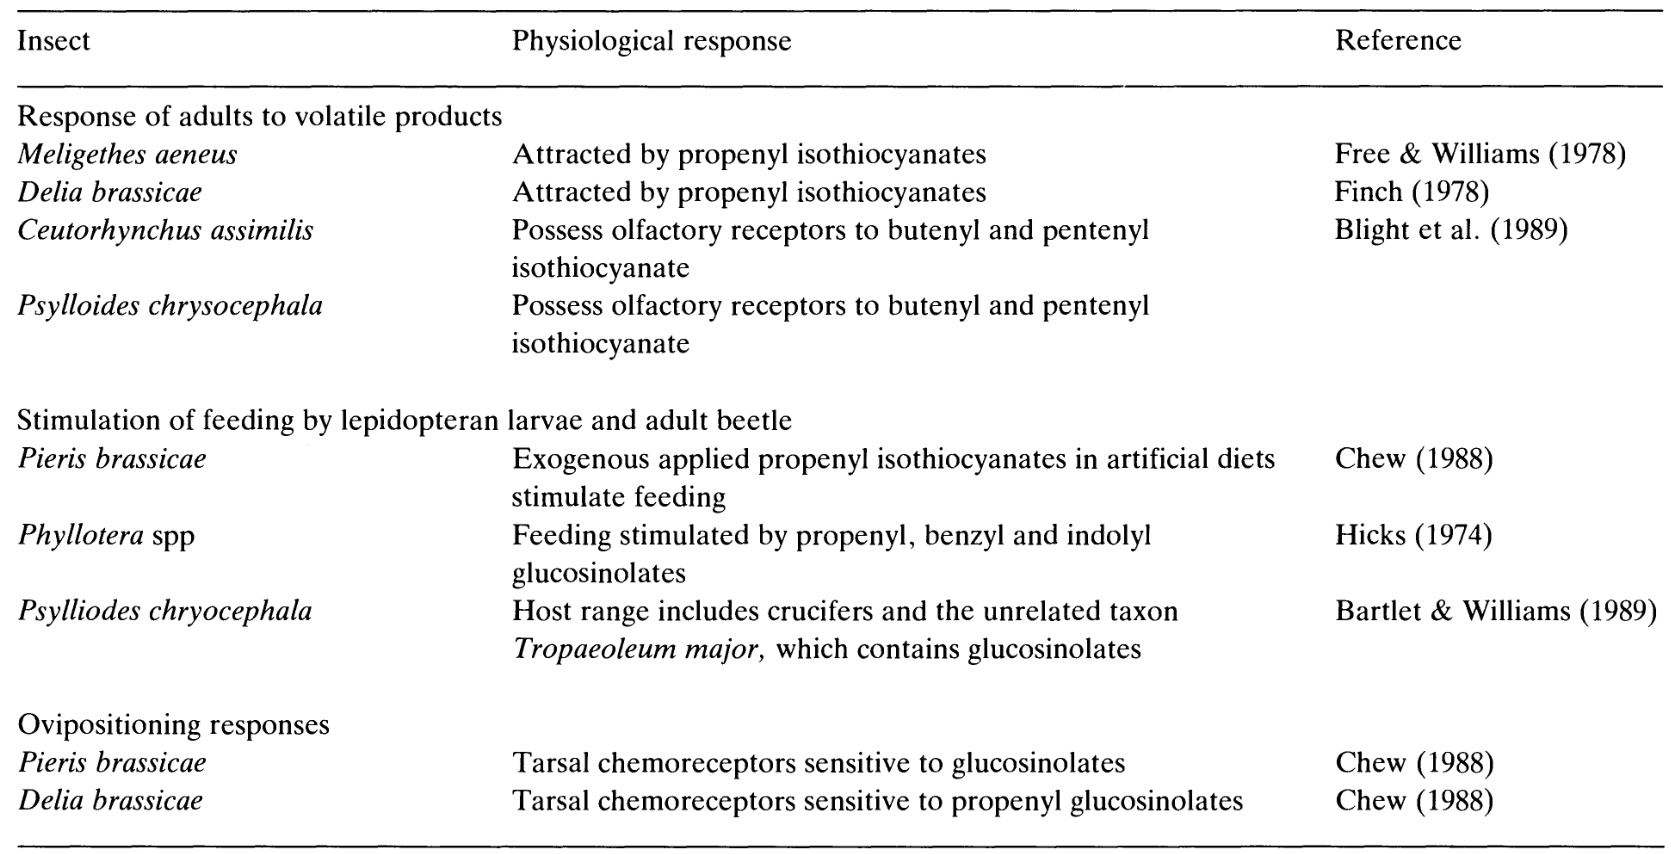
\includegraphics[width=0.66\linewidth]{../images/insect_glucosinolate_signalling} \end{center}

\vspace{-0.5cm}

\begin{itemize}
\tightlist
\item
  Besides interacting with insects,

  \begin{itemize}
  \tightlist
  \item
    isothiocyanates (a constituent in brassica) are toxic to
    \emph{Peronospora parasitica}, \emph{Mycosphaerella brassicae} and
    \emph{Alternaria} spp.
  \end{itemize}
\end{itemize}

\end{small}
\end{frame}

\hypertarget{breeding-for-disease-resistance}{%
\section{Breeding for Disease
Resistance}\label{breeding-for-disease-resistance}}

\begin{frame}{Epidemiology and forcasting}
\protect\hypertarget{epidemiology-and-forcasting}{}
\begin{figure}
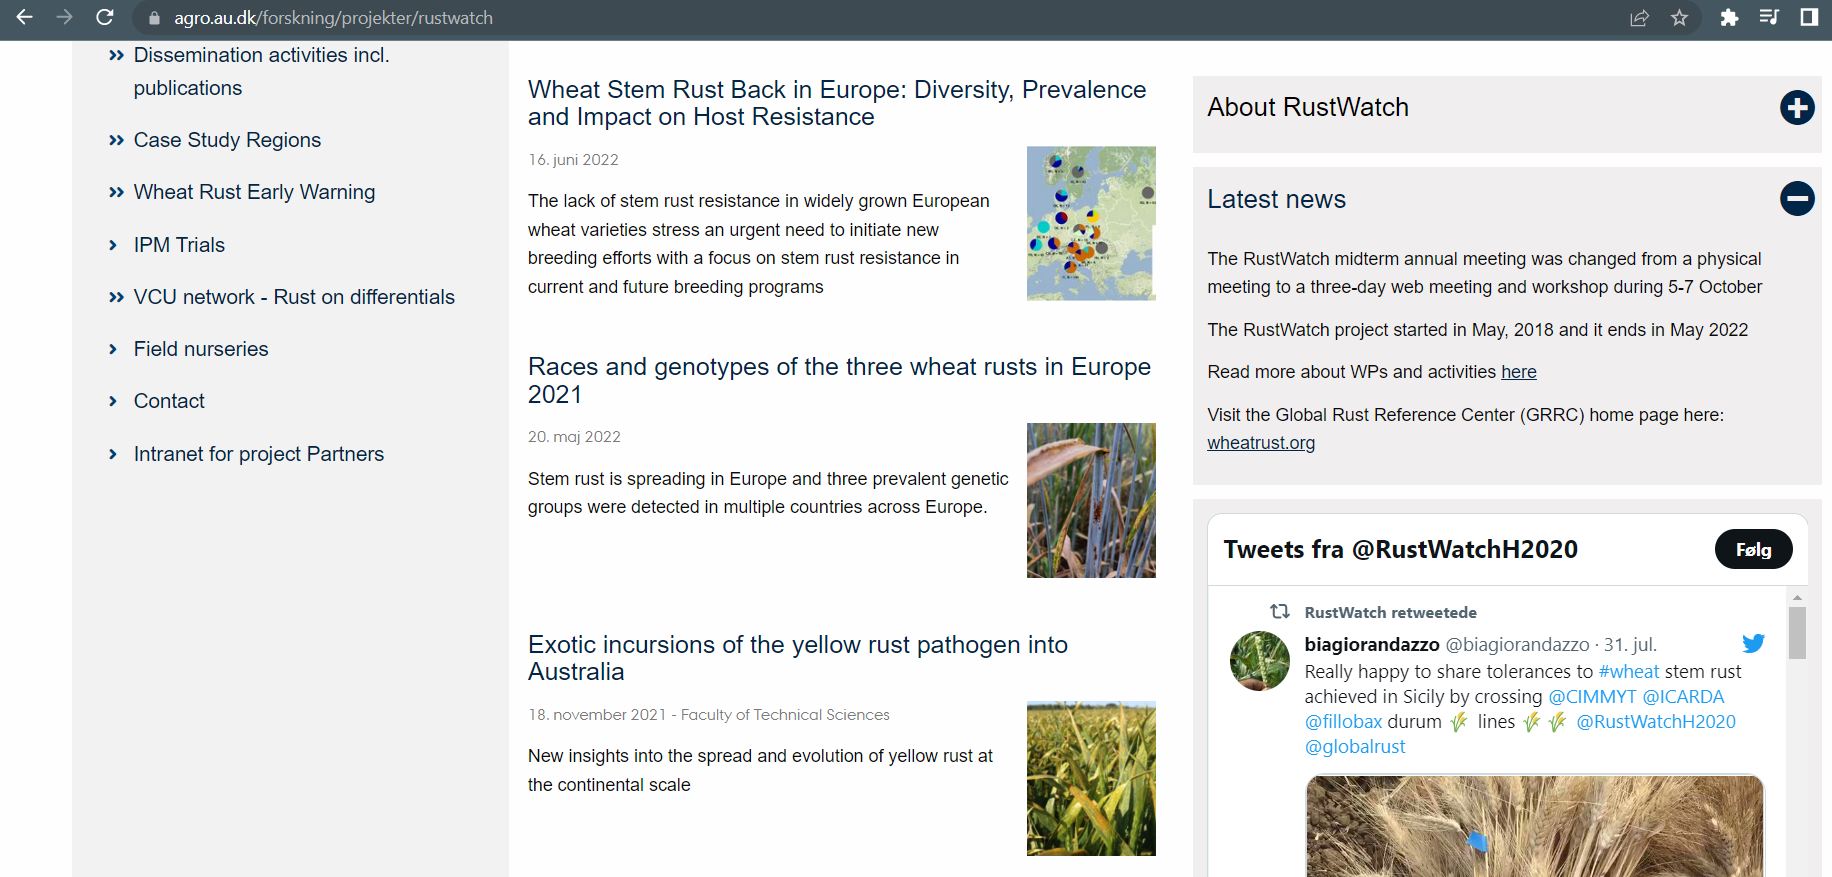
\includegraphics[width=0.95\linewidth]{../images/rust_epidemiology_networking_forcasting} \caption{A early-warning system to improve preparedness and resilience to emerging rust diseases on wheat, based on Europe by monitoring rust populations -- identification, and investigation of virulence, agressiveness and adaptation to warmer temperatures.}\label{fig:rust-epidemiology-network}
\end{figure}
\end{frame}

\hypertarget{bibliography}{%
\section{Bibliography}\label{bibliography}}

\begin{frame}{References}
\protect\hypertarget{references}{}
\end{frame}




\end{document}
